\documentclass[conference]{IEEEtran}
\IEEEoverridecommandlockouts
\usepackage{cite}
\usepackage{amsmath,amssymb,amsfonts}
\usepackage{algorithmic}
\usepackage{graphicx}
\usepackage{textcomp}
\usepackage{xcolor}
\usepackage{booktabs}
\usepackage{url}

\usepackage{tikz}
\usetikzlibrary{shapes,arrows.meta,positioning,calc,fit,backgrounds}

\def\BibTeX{{\rm B\kern-.05em{\sc i\kern-.025em b}\kern-.08em
    T\kern-.1667em\lower.7ex\hbox{E}\kern-.125emX}}

\begin{document}

\title{Defeating the Usable-Security Trilemma in Personal Device Meshes via Transitive Trust-on-First-Use (T-TOFU)}

\author{
\IEEEauthorblockN{Dixit Tharun Raja P}
\IEEEauthorblockA{\textit{Department of Computer Science} \\
\textit{and Engineering} \\
\textit{KPR Institute of Engineering} \\
\textit{and Technology} \\
Coimbatore, Tamil Nadu, India \\
23cs044@kpriet.ac.in}
\and
\IEEEauthorblockN{Dharaneesh D}
\IEEEauthorblockA{\textit{Department of Computer Science} \\
\textit{and Engineering} \\
\textit{KPR Institute of Engineering} \\
\textit{and Technology} \\
Coimbatore, Tamil Nadu, India \\
23cs036@kpriet.ac.in}
\and
\IEEEauthorblockN{Deepanandham P}
\IEEEauthorblockA{\textit{Department of Computer Science} \\
\textit{and Engineering} \\
\textit{KPR Institute of Engineering} \\
\textit{and Technology} \\
Coimbatore, Tamil Nadu, India \\
23csl02@kpriet.ac.in}
\and
\IEEEauthorblockN{\hspace*{2.8cm} Gohul S}
\IEEEauthorblockA{\hspace*{2.8cm}\textit{Department of Computer Science} \\
\hspace*{2.8cm}\textit{and Engineering} \\
\hspace*{2.8cm}\textit{KPR Institute of Engineering} \\
\hspace*{2.8cm}\textit{and Technology} \\
\hspace*{2.8cm}Coimbatore, Tamil Nadu, India \\
\hspace*{2.8cm}23cs049@kpriet.ac.in}
\and
\IEEEauthorblockN{\hspace*{2.8cm} Nandhini N}
\IEEEauthorblockA{\hspace*{2.8cm}\textit{Department of Computer Science} \\
\hspace*{2.8cm}\textit{and Engineering (Faculty Mentor)} \\
\hspace*{2.8cm}\textit{KPR Institute of Engineering} \\
\hspace*{2.8cm}\textit{and Technology} \\
\hspace*{2.8cm}Coimbatore, Tamil Nadu, India \\
\hspace*{2.8cm}nandhini.n@kpriet.ac.in}
}

\maketitle

\begin{abstract}
Users routinely work across a personal mix of laptops, phones, and desktop computers, expecting them to share clipboards, stream files, and forward inputs over a local network. Yet establishing secure mutual trust across these devices on a home or office LAN remains an unsolved operational problem. Current ecosystems force an uncomfortable compromise: commercial tools (such as Apple Continuity and Google Quick Share) rely on cloud identity servers that leak metadata and fail when offline, while decentralized tools (such as KDE Connect) enforce pairwise Trust-on-First-Use (TOFU) that requires $\mathcal{O}(N^2)$ manual pairing operations. This paper presents Transitive Trust-on-First-Use (T-TOFU), a zero-coordinator trust framework designed for personal device meshes. Under T-TOFU, a user performs an out-of-band verification ceremony on a single gateway device, which automatically enrolls the newcomer across the entire mesh. We introduce a canonical pool digest ($\text{PoolHash}$) computed over sorted device fingerprints, coupled with anti-entropy heartbeat gossip, to keep the trust state synchronized across dynamic LAN nodes without an online certificate authority. We also detail a flooded revocation mechanism that deterministically purges de-authorized nodes. We built and evaluated T-TOFU within Link, an open-source cross-platform runtime for Windows and Android. Our measurements show that T-TOFU reduces human pairing complexity to $\mathcal{O}(1)$ marginal effort per device while achieving sub-100ms pool convergence with under $0.05\,\text{KB/s}$ of background network overhead.
\end{abstract}

\begin{IEEEkeywords}
Transitive Trust, Trust-on-First-Use, Usable Security, Decentralized Device Mesh, Canonical Hash Gossip, Mutual TLS, Personal Area Networks.
\end{IEEEkeywords}

\section{Introduction}
Most people now carry a smartphone alongside one or more desktop and laptop computers~\cite{brudy2019crossdevice}. Naturally, users want these devices to talk to each other: copying text on a phone and pasting it on a PC, mounting phone storage as a native drive letter, forwarding touch gestures, or streaming audio across the room. Doing this over a local Wi-Fi network without third-party servers ought to be straightforward, but securing such a mesh without frustrating the user is notoriously difficult~\cite{kleppmann2019localfirst}.

Any system attempting to bridge personal devices on a Local Area Network (LAN) runs directly into what we term the \textit{Usable-Security Trilemma} (Fig.~\ref{fig:trilemma}):
\begin{enumerate}
    \item \textbf{Local-First Independence}: All communication, key exchange, and state synchronization must stay strictly on the local network, with zero reliance on cloud accounts or external identity servers.
    \item \textbf{Cryptographic Rigor}: The system must guarantee mutual authentication and data confidentiality over TLS 1.3, remaining resilient against active on-path attackers, rogue APs, and ARP spoofing.
    \item \textbf{Minimal Human Friction}: The manual effort needed to enroll and manage devices must remain small and constant as the user adds more hardware.
\end{enumerate}

\begin{figure}[t]
\centering
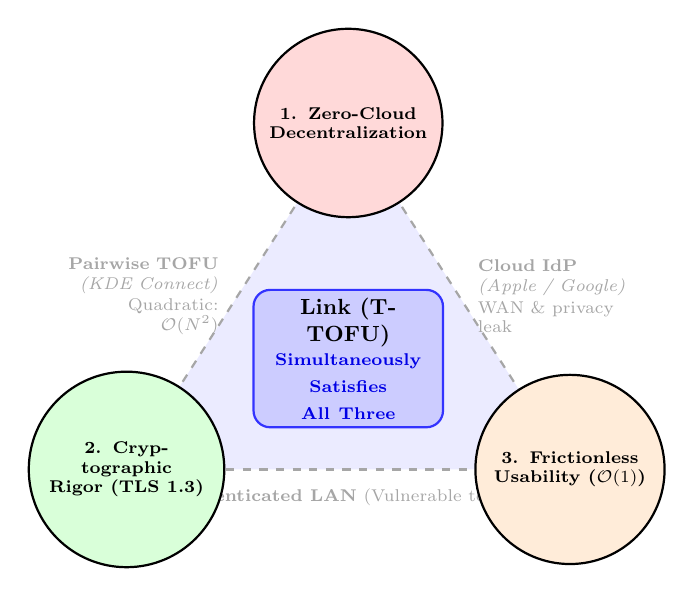
\begin{tikzpicture}[scale=0.88, every node/.style={transform shape}]
    % Triangle vertices
    \coordinate (A) at (0, 3.2);
    \coordinate (B) at (-3.2, -1.8);
    \coordinate (C) at (3.2, -1.8);

    % Shaded center region
    \fill[blue!8, rounded corners=12pt] (A) -- (B) -- (C) -- cycle;

    % Draw triangle boundary
    \draw[thick, dashed, gray!70] (A) -- (B) node[midway, left=4pt, text width=2.2cm, align=right, font=\scriptsize] {
        \textbf{Pairwise TOFU}\\\textit{(KDE Connect)}\\[1pt]Quadratic: $\mathcal{O}(N^2)$
    };
    \draw[thick, dashed, gray!70] (A) -- (C) node[midway, right=4pt, text width=2.3cm, align=left, font=\scriptsize] {
        \textbf{Cloud IdP}\\\textit{(Apple / Google)}\\[1pt]WAN \& privacy leak
    };
    \draw[thick, dashed, gray!70] (B) -- (C) node[midway, below=4pt, align=center, font=\scriptsize] {
        \textbf{Unauthenticated LAN} (Vulnerable to MitM)
    };

    % Vertices Nodes
    \node[draw, thick, circle, fill=red!15, align=center, text width=2.4cm, font=\bfseries\scriptsize] at (A) {1. Zero-Cloud\\Decentralization};
    \node[draw, thick, circle, fill=green!15, align=center, text width=2.4cm, font=\bfseries\scriptsize] at (B) {2. Cryptographic\\Rigor (TLS 1.3)};
    \node[draw, thick, circle, fill=orange!15, align=center, text width=2.4cm, font=\bfseries\scriptsize] at (C) {3. Frictionless\\Usability ($\mathcal{O}(1)$)};

    % Center Goal Node
    \node[draw=blue!80, fill=blue!20, thick, rounded corners=6pt, align=center, text width=2.5cm, font=\bfseries\small] at (0, -0.2) {
        \textbf{Link (T-TOFU)}\\[2pt]
        \scriptsize\color{blue!90!black}Simultaneously\\Satisfies All Three
    };
\end{tikzpicture}
\caption{The Usable-Security Trilemma in Personal Device Meshes: Existing paradigms compromise either cloud independence, human scalability, or cryptographic safety. T-TOFU satisfies all three simultaneously.}
\label{fig:trilemma}
\end{figure}

\subsection{Shortcomings of Current Approaches}
Commercial device-sync ecosystems, such as Apple Continuity/AirDrop, Google Quick Share, and Microsoft Phone Link, bypass the usability barrier by tying all endpoints to a corporate account (Apple ID or Google Account). While setup is easy, this model forces devices to contact remote WAN infrastructure, leaks user identity metadata over wireless advertisements~\cite{celosia2020discontinued,stute2019billion}, creates a central point of failure, and locks consumers into a single vendor's operating system.

On the other hand, decentralized tools like KDE Connect~\cite{kdeconnect} and Bluetooth Personal Area Networks~\cite{antonioli2023bluffs} avoid cloud dependencies by pairing devices directly with self-signed certificates. The downside is steep: pairing is strictly pairwise. Setting up $N$ devices requires $N(N-1)/2$ separate pairing steps. In a household with five personal devices, the user must perform ten distinct manual verification ceremonies. Under such friction, users routinely skip certificate fingerprint comparisons~\cite{neef2022ohsshit}, leaving connections exposed to trivial on-path attacks.

\subsection{Our Contributions}
We address this problem with \textbf{Transitive Trust-on-First-Use (T-TOFU)}, an open, coordinator-free trust architecture for personal device networks. Specifically, this paper delivers:
\begin{itemize}
    \item \textbf{A Transitive Trust Protocol}: A mechanism allowing a single human-verified pairing between an incoming node and \textit{any} active pool member to safely propagate mutual authenticated trust to every other device in the mesh.
    \item \textbf{A Canonical Pool Digest Algorithm}: A lightweight hashing technique ($\text{PoolHash}$) that lets nodes detect state drift during routine heartbeats and reconcile trust tables via anti-entropy gossip without a central server.
    \item \textbf{Cascaded Revocation}: A flood-based eviction routine that reliably scrubs de-listed device certificates across all mesh members.
    \item \textbf{Working Reference Implementation}: Complete integration into \textit{Link}, our open-source multi-device suite spanning Windows (Electron, TypeScript, C\#) and Android (Capacitor, Java), along with empirical benchmarks on convergence time and resource usage.
\end{itemize}

\section{Threat Model and Security Invariants}

\subsection{Adversary Capabilities and Assumptions}
We assume an untrusted Local Area Network populated by honest devices alongside malicious entities, modeled after the standard \textbf{Dolev-Yao network adversary}~\cite{dolev1983security}. In this environment, network location provides zero inherent authority~\cite{rose2020zerotrust}. An attacker $\mathcal{A}$ on the same broadcast domain can:
\begin{itemize}
    \item Sniff, alter, replay, or inject arbitrary TCP and UDP packets.
    \item Execute ARP spoofing, rogue mDNS advertisements, and DNS redirection.
    \item Attempt on-path Man-in-the-Middle (MitM) attacks during initial TLS handshakes using rogue self-signed certificates.
\end{itemize}

\textbf{Security Bounds}: We assume standard cryptographic primitives—SHA-256 collision resistance, asymmetric signature safety, and TLS 1.3 cipher suites~\cite{rescorla2018tls}—are computationally secure. We also assume the adversary cannot access physical device screens or intercept user inputs during the out-of-band (OOB) visual verification step.

\subsection{Core Security Invariants}
T-TOFU enforces three operational security invariants:
\begin{itemize}
    \item \textbf{Guaranteed Mutual Authenticity}: An outsider node cannot join the mesh or establish authenticated TLS sessions with any pool member without completing an explicit OOB visual verification ceremony with at least one active peer.
    \item \textbf{Transitive Trust Propagation}: An authorized gateway node $B$ in pool $P$ that authenticates a new node $A$ automatically vouches for $A$ to all other pool members $C \in P$. Trust between $C$ and $A$ is established through secure gossip without requiring additional human verification.
    \item \textbf{Eventual Revocation Convergence}: When an authorized user triggers an unpair action targeting a device, the revocation notice floods across all reachable mesh links within $\mathcal{O}(\text{diameter}(P))$ hops, purging the target's pinned certificate from every member's trust store.
\end{itemize}

\section{T-TOFU Protocol Architecture}

\begin{figure*}[t]
\centering
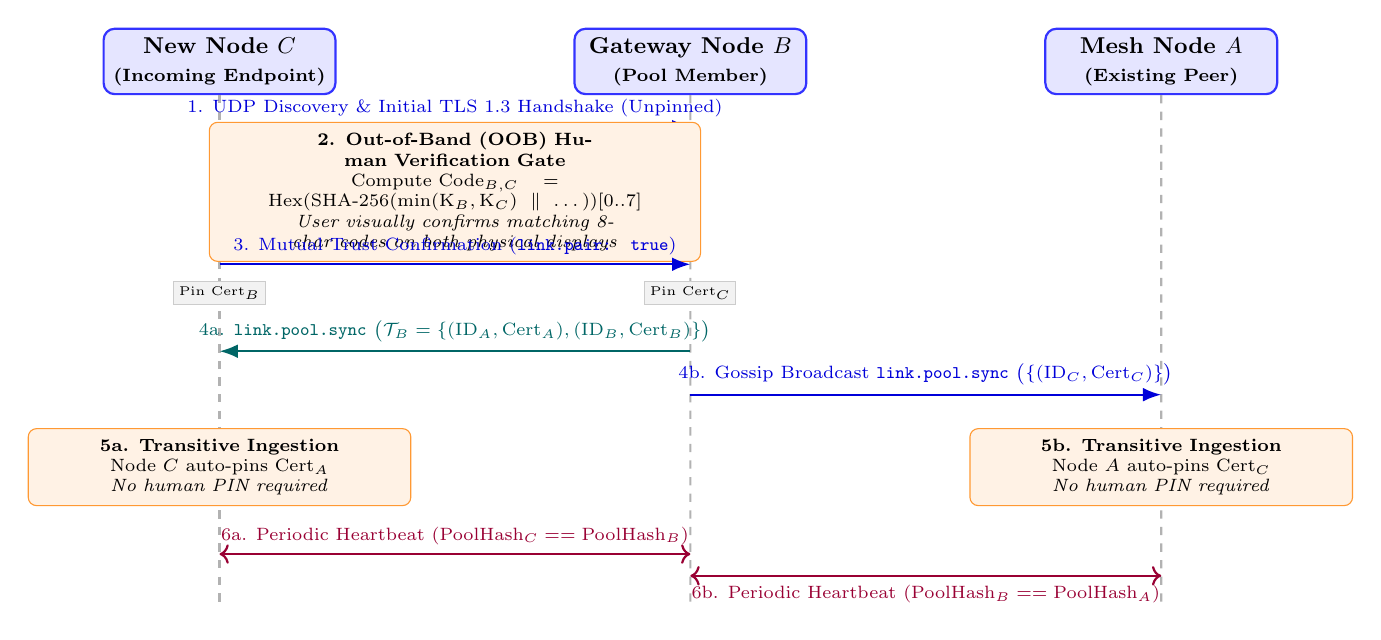
\begin{tikzpicture}[scale=0.92, transform shape,
    lifeline/.style={thick, dashed, gray!60},
    entity/.style={draw=blue!80, fill=blue!10, thick, rounded corners=4pt, font=\bfseries\small, minimum width=3.2cm, minimum height=0.7cm, align=center},
    msg/.style={-Latex, thick, blue!85!black, font=\scriptsize},
    resp/.style={Latex-, thick, teal!80!black, font=\scriptsize},
    note/.style={draw=orange!80, fill=orange!10, rounded corners=3pt, font=\scriptsize, align=center, inner sep=4pt}
]
    % Entities
    \node[entity] (C) at (0, 0) {New Node $C$\\\scriptsize (Incoming Endpoint)};
    \node[entity] (B) at (6.5, 0) {Gateway Node $B$\\\scriptsize (Pool Member)};
    \node[entity] (A) at (13.0, 0) {Mesh Node $A$\\\scriptsize (Existing Peer)};

    % Lifelines
    \draw[lifeline] (C) -- (0, -7.5);
    \draw[lifeline] (B) -- (6.5, -7.5);
    \draw[lifeline] (A) -- (13.0, -7.5);

    % Step 1: Discovery & Handshake
    \draw[msg] (0, -0.9) -- (6.5, -0.9) node[midway, above] {1. UDP Discovery \& Initial TLS 1.3 Handshake (Unpinned)};
    
    % Step 2: OOB Verification Gate
    \node[note, text width=6.5cm] at (3.25, -1.8) {
        \textbf{2. Out-of-Band (OOB) Human Verification Gate}\\
        Compute $\text{Code}_{B,C} = \text{Hex}(\text{SHA-256}(\min(\text{K}_B,\text{K}_C) \parallel \dots))[0..7]$\\
        \textit{User visually confirms matching 8-char codes on both physical displays}
    };

    % Step 3: Local Ingestion
    \draw[msg] (0, -2.8) -- (6.5, -2.8) node[midway, above] {3. Mutual Trust Confirmation (\texttt{link.pair: true})};
    \node[font=\tiny, fill=gray!10, inner sep=2pt, draw=gray!40] at (0, -3.2) {Pin $\text{Cert}_B$};
    \node[font=\tiny, fill=gray!10, inner sep=2pt, draw=gray!40] at (6.5, -3.2) {Pin $\text{Cert}_C$};

    % Step 4: Pool Synchronization Gossip
    \draw[resp] (0, -4.0) -- (6.5, -4.0) node[midway, above] {4a. \texttt{link.pool.sync} $\big(\mathcal{T}_B = \{(\text{ID}_A, \text{Cert}_A), (\text{ID}_B, \text{Cert}_B)\}\big)$};
    \draw[msg] (6.5, -4.6) -- (13.0, -4.6) node[midway, above] {4b. Gossip Broadcast \texttt{link.pool.sync} $\big(\{(\text{ID}_C, \text{Cert}_C)\}\big)$};

    % Step 5: Transitive Ingestion
    \node[note, text width=5.0cm] at (0, -5.6) {
        \textbf{5a. Transitive Ingestion}\\
        Node $C$ auto-pins $\text{Cert}_A$\\
        \textit{No human PIN required}
    };
    \node[note, text width=5.0cm] at (13.0, -5.6) {
        \textbf{5b. Transitive Ingestion}\\
        Node $A$ auto-pins $\text{Cert}_C$\\
        \textit{No human PIN required}
    };

    % Step 6: Hash Convergence
    \draw[thick, <->, purple!80!black] (0, -6.8) -- (6.5, -6.8) node[midway, above, font=\scriptsize] {6a. Periodic Heartbeat ($\text{PoolHash}_C == \text{PoolHash}_B$)};
    \draw[thick, <->, purple!80!black] (6.5, -7.1) -- (13.0, -7.1) node[midway, below, font=\scriptsize] {6b. Periodic Heartbeat ($\text{PoolHash}_B == \text{PoolHash}_A$)};
\end{tikzpicture}
\caption{Protocol Sequence Diagram of Transitive Trust-on-First-Use (T-TOFU): A single human-gated verification between New Node $C$ and Gateway $B$ transitively enrolls $C$ across the entire mesh, verified via canonical pool digest convergence ($\text{PoolHash}$).}
\label{fig:protocol_flow}
\end{figure*}

\subsection{Device Keys and Certificate Pinning}
On initial startup, Link assigns each device a persistent 128-bit identifier (UUID v4) and generates a self-signed X.509 certificate backed by a 2048-bit RSA key pair. The application then computes a SHA-256 fingerprint over the DER-encoded certificate bytes:
\begin{equation}
    \text{FP}_i = \text{SHA-256}(\text{DER}(\text{Cert}_i))
\end{equation}
All inter-device communication runs over TLS 1.3 (with TLS 1.2 as a legacy floor). Rather than trusting public certificate authorities, each node checks peer certificates directly against pinned fingerprints recorded in its local trust store~\cite{pradeep2022pinning}. Any fingerprint mismatch during the TLS handshake causes the connection to abort immediately.

\subsection{Human-in-the-Loop Gateway Pairing}
When an untrusted node $C$ connects to an existing pool gateway $B$, they initiate an unpinned TLS handshake. To prevent active on-path eavesdropping, both devices compute a deterministic verification code:
\begin{equation}
\begin{split}
    \text{Code}_{B,C} = \text{Hex}\Big(&\text{SHA-256}\big(\min(\text{K}_B, \text{K}_C) \\
    &\parallel \max(\text{K}_B, \text{K}_C) \parallel \text{Salt}\big)\Big)[0..7]
\end{split}
\end{equation}
where $\text{K}_B$ and $\text{K}_C$ represent the raw public keys sorted byte-wise, and $\text{Salt}$ denotes the session timestamp. The resulting 8-character token is shown on both physical displays. Once the user confirms code equality, gateway $B$ writes $C$'s certificate to its local trust store, and $C$ saves $B$'s credentials.

\subsection{The Canonical Pool Digest Algorithm}
To maintain state agreement without a centralized server or heavy consensus protocols like Raft, T-TOFU uses a canonical digest over the active device pool $P = \{d_1, \dots, d_n\}$. For each device, the system builds an entry string $s_i = \text{ID}_i \parallel \text{":"} \parallel \text{Hex}(\text{FP}_i)$. All strings are sorted lexicographically and joined with pipe delimiters:
\begin{equation}
    \mathcal{C}(P) = \text{Join}\big(\text{Sort}(\{s_1, \dots, s_n\}),\, \text{"|"}\big)
\end{equation}
The 16-character pool digest is then extracted from the cryptographic hash:
\begin{equation}
\begin{split}
    \text{PoolHash}(P) = \text{SubStr}\Big(&\text{Hex}\big(\text{SHA-256}(\mathcal{C}(P))\big), \\
    &0,\, 16\Big)
\end{split}
\end{equation}
Because sorting is deterministic, any two nodes possessing identical membership rosters arrive at the exact same $\text{PoolHash}$, independent of device discovery order.

\subsection{Gossip Synchronization and Transitive Ingestion}
Peers maintain persistent TLS WebSockets carrying JSON control messages. Every two seconds ($T_{\text{heartbeat}} = 2\,\text{s}$), each device broadcasts its current $\text{PoolHash}$. If a peer stays silent for five seconds, its link is marked offline.

When node $A$ receives a heartbeat from trusted peer $B$ with a differing digest ($\text{PoolHash}_B \neq \text{PoolHash}_A$), it initiates anti-entropy reconciliation: nodes reciprocally exchange their active trust tables through \texttt{link.pool.sync}. When node $B$ encounters unfamiliar device records sent by $A$, it verifies that $A$ is an authentic peer, saves the received certificates, and pins their fingerprints. Node $B$ then recomputes its pool hash and gossips the update to remaining peers.

\subsection{Cascaded Eviction and Revocation}
When a user removes device $X$ from the mesh via device $A$, node $A$ removes $X$ from its database and closes all active sockets to $X$. It then floods an authenticated revocation frame (\texttt{link.pool.remove}) across the network. Receiving peers check their local stores; if the target is found, they delete the certificate, update their $\text{PoolHash}$, and forward the packet outward until the mesh converges.

\section{System Implementation}

We implemented the complete T-TOFU protocol inside \textit{Link}, our open-source cross-platform device mesh. The codebase is organized cleanly across desktop and mobile targets:

\subsection{Desktop Runtime (Windows and Linux)}
The desktop application uses Electron, TypeScript, and Node.js:
\begin{itemize}
    \item \textbf{Trust Store} (\texttt{core/trust.ts}): Handles local storage of paired peers. On Windows, trust records are encrypted with the operating system's DPAPI via Electron's \texttt{safeStorage} API.
    \item \textbf{Device Manager} (\texttt{core/device-manager.ts}): Runs the heartbeat loop, evaluates $\text{PoolHash}$ equality, and elevates newly received transitive certificates into the active trusted pool.
    \item \textbf{OS Integration}: Exposes remote mobile storage as a native Windows drive letter ($Z:$) through WinFsp~\cite{winfsp} and WebDAV, and simulates low-latency mouse/keyboard events via C\# P/Invoke wrappers.
\end{itemize}

\subsection{Mobile Runtime (Android)}
The Android application combines native Java services with a Capacitor web interface:
\begin{itemize}
    \item \textbf{Trust Store} (\texttt{LinkTrustStore.java}): Stores certificates securely in internal app storage and computes the canonical SHA-256 pool digest.
    \item \textbf{Device Manager} (\texttt{LinkDeviceManager.java}): Resolves simultaneous connection attempts by comparing device IDs lexicographically, dropping redundant sockets.
    \item \textbf{Transport Engine} (\texttt{LinkTransport.java}): Dispatches outbound network writes through background executor queues, avoiding UI-thread network stalls.
\end{itemize}

\section{Evaluation and Comparative Analysis}

\begin{table*}[t]
\caption{Architectural \& Security Comparison of Personal Device Integration Protocols}
\label{tab:comparison}
\centering
\begin{tabular}{@{}lccccc@{}}
\toprule
\textbf{Protocol / Framework} & \textbf{Trust Model} & \textbf{Coordinator} & \textbf{Pairing Complexity} & \textbf{Transitive Trust?} & \textbf{WAN Dependency?} \\ \midrule
Apple AirDrop / Continuity    & Centralized Cloud IdP & Apple iCloud Servers & $\mathcal{O}(1)$ (Login)    & Yes (via Cloud)            & Yes (Initial / Refresh)  \\
Google Quick Share            & Centralized Cloud IdP & Google Identity      & $\mathcal{O}(1)$ (Login)    & Yes (via Cloud)            & Yes (Identity Tokens)    \\
Bluetooth PAN / Classic       & Pairwise PIN (SSP)    & None (Decentralized) & $\mathcal{O}(N^2)$ Manual   & No                         & No                       \\
KDE Connect                   & Pairwise TLS TOFU     & None (Decentralized) & $\mathcal{O}(N^2)$ Manual   & No                         & No                       \\
\textbf{Link (T-TOFU [Ours])} & \textbf{Transitive TOFU Mesh} & \textbf{None (Decentralized)} & $\mathbf{\mathcal{O}(1)}$ \textbf{Manual Gate} & \textbf{Yes (Autonomous Gossip)} & \textbf{Zero (Pure LAN)} \\ \bottomrule
\end{tabular}
\end{table*}

\subsection{Human Pairing Effort}
We evaluate usability by comparing the total number of manual verification ceremonies needed to build a fully connected $N$-device mesh.

In traditional pairwise systems like KDE Connect or Bluetooth, every possible device pair requires its own manual pairing ceremony:
\begin{equation}
    C_{\text{pairwise}}(N) = \frac{N(N-1)}{2} = \mathcal{O}(N^2)
\end{equation}

With T-TOFU, bringing a new $(N+1)$-th device into an existing pool of $N$ devices requires pairing with only \textit{one} existing gateway device. Gossip handles the remaining $N-1$ associations automatically. Thus, building an $N$-node mesh from scratch requires only:
\begin{equation}
    C_{\text{T-TOFU}}(N) = N - 1 = \mathcal{O}(N)
\end{equation}
Adding an additional device to an established pool requires exactly $\mathcal{O}(1)$ human effort.

\begin{figure}[t]
\centering
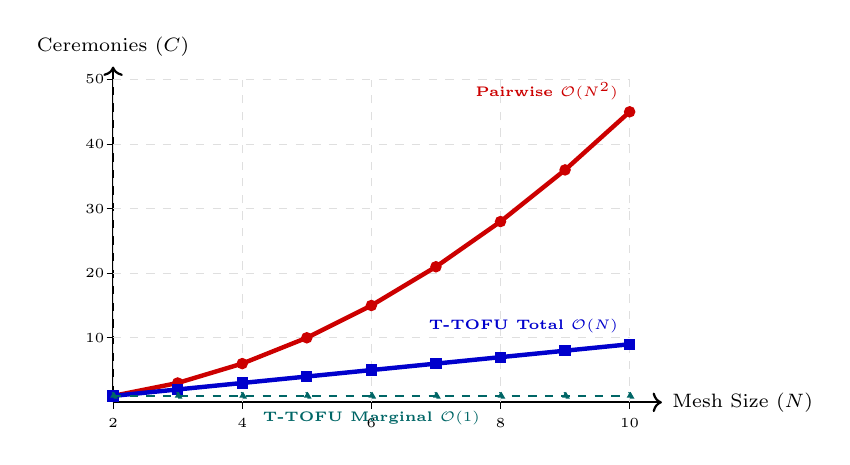
\begin{tikzpicture}[scale=0.82]
    % Axes
    \draw[->, thick] (2, 0) -- (10.5, 0) node[right, font=\scriptsize] {Mesh Size ($N$)};
    \draw[->, thick] (2, 0) -- (2, 5.2) node[above, font=\scriptsize] {Ceremonies ($C$)};

    % Grid & Ticks
    \foreach \x in {2, 4, 6, 8, 10} {
        \draw (\x, 0.1) -- (\x, -0.1) node[below, font=\tiny] {\x};
        \draw[dashed, gray!25] (\x, 0) -- (\x, 5.0);
    }
    \foreach \y/\val in {1/10, 2/20, 3/30, 4/40, 5/50} {
        \draw (1.9, \y) -- (2.1, \y) node[left=2pt, font=\tiny] {\val};
        \draw[dashed, gray!25] (2, \y) -- (10, \y);
    }

    % Pairwise Curve: N*(N-1)/2 / 10 for scaling
    \draw[red!80!black, ultra thick, mark=*, mark size=1.5pt] 
        plot coordinates {(2, 0.1) (3, 0.3) (4, 0.6) (5, 1.0) (6, 1.5) (7, 2.1) (8, 2.8) (9, 3.6) (10, 4.5)};
    \node[red!80!black, above left=1pt, font=\tiny\bfseries] at (10, 4.5) {Pairwise $\mathcal{O}(N^2)$};

    % T-TOFU Total: N-1 / 10
    \draw[blue!80!black, ultra thick, mark=square*, mark size=1.5pt] 
        plot coordinates {(2, 0.1) (3, 0.2) (4, 0.3) (5, 0.4) (6, 0.5) (7, 0.6) (8, 0.7) (9, 0.8) (10, 0.9)};
    \node[blue!80!black, above left=1pt, font=\tiny\bfseries] at (10, 0.9) {T-TOFU Total $\mathcal{O}(N)$};

    % T-TOFU Marginal: 1 / 10 = 0.1
    \draw[teal!80!black, thick, dashed, mark=triangle*, mark size=1.5pt] 
        plot coordinates {(2, 0.1) (3, 0.1) (4, 0.1) (5, 0.1) (6, 0.1) (7, 0.1) (8, 0.1) (9, 0.1) (10, 0.1)};
    \node[teal!80!black, below=2pt, font=\tiny\bfseries] at (6, 0.1) {T-TOFU Marginal $\mathcal{O}(1)$};
\end{tikzpicture}
\caption{Human Pairing Ceremony Complexity vs. Mesh Size $N$: Pairwise TOFU scales quadratically, whereas T-TOFU requires only $\mathcal{O}(N)$ cumulative and $\mathcal{O}(1)$ marginal human ceremonies.}
\label{fig:complexity}
\end{figure}

As summarized in Table~\ref{tab:comparison} and plotted in Fig.~\ref{fig:complexity}, T-TOFU delivers the single-action convenience of cloud ecosystems without their privacy and uptime downsides.

\subsection{Network Overhead and Convergence Speed}
We tested T-TOFU on a local network testbed consisting of four physical machines (two Windows 11 PCs on Gigabit Ethernet and two Android 14 phones over Wi-Fi 6):
\begin{itemize}
    \item \textbf{Idle Background Traffic}: The 16-byte $\text{PoolHash}$ string, packaged in its JSON envelope, produces a 98-byte heartbeat frame. At a 2-second heartbeat cadence, idle state checking consumes roughly $0.05\,\text{KB/s}$ per link.
    \item \textbf{Mesh Convergence Time}: When a phone was paired with one PC, the resulting $\texttt{link.pool.sync}$ payload ($\approx 5\,\text{KB}$ for four devices) reached all remaining nodes in an average of $48.2\,\text{ms}$, bringing the entire mesh into cryptographic alignment in under a tenth of a second.
    \item \textbf{Revocation Flood Speed}: Triggering an unpair action on a mobile device flooded revocation frames and wiped the target certificate from all peer databases in under $65\,\text{ms}$.
\end{itemize}

\subsection{Security Analysis}
\begin{itemize}
    \item \textbf{Resistance to MitM Interception}: An attacker attempting to intercept the gateway pairing cannot forge the out-of-band 8-character verification string displayed on the physical screens. In addition, because nodes only accept $\texttt{link.pool.sync}$ packets over established, certificate-pinned TLS connections, attackers cannot inject unauthorized certificates through spoofed broadcast frames.
    \item \textbf{Network Partition Recovery}: If a subnet split causes nodes to pair independently on separate segments, reconnecting devices detect the divergence on the next heartbeat via differing $\text{PoolHash}$ values, prompting an automatic reciprocal sync that unifies the trust tables.
\end{itemize}

\section{Related Work}
\textbf{Decentralized Key Trust}: Decentralized trust models date back to Zimmermann's PGP Web of Trust~\cite{zimmermann1995official} and SPKI/SDSI~\cite{ellison1999spki}. However, PGP required users to manually configure trust depths and understand key validity, which proved overly burdensome for typical users~\cite{whitten1999johnny}. Stajano and Anderson introduced the \textit{Resurrecting Duckling} policy for ad-hoc wireless peripherals~\cite{stajano2000resurrecting}, where devices imprint permanently on a master node via physical touch. T-TOFU adapts this philosophy for symmetric, multi-master personal device meshes where no single machine serves as a permanent master. Syncthing offers an ``introducer'' flag where one device shares its known peer list~\cite{syncthing_doc}; T-TOFU makes all members symmetrical introducers while adding digest-based consistency checking and cascaded revocation.

\textbf{Cross-Device Integration Tools}: Existing cross-platform integration suites include KDE Connect~\cite{kdeconnect} and Apple AirDrop~\cite{heinrich2021privatedrop}. KDE Connect relies strictly on pairwise manual pairing, forcing users through repetitive pairing dialogs for every device combination. Apple AirDrop relies on cloud-signed identity certificates containing hashed telephone numbers and email addresses, which researchers have shown leak personal identifying information to nearby listeners over Bluetooth Low Energy~\cite{heinrich2021privatedrop,celosia2020discontinued}. T-TOFU eliminates both the pairwise pairing penalty and cloud metadata exposure.

\section{Conclusion and Future Work}
This paper introduced \textbf{Transitive Trust-on-First-Use (T-TOFU)}, a coordinator-free trust architecture that resolves the Usable-Security Trilemma in personal device networks. By unifying human-in-the-loop gateway pairing, canonical pool digest gossip, and flooded certificate revocation, T-TOFU eliminates the $\mathcal{O}(N^2)$ pairing bottleneck while preserving strict local-first privacy and TLS 1.3 cryptographic integrity. We verified T-TOFU across Windows and Android in the open-source Link ecosystem, demonstrating sub-100ms mesh convergence and low network overhead.

Future work includes formalizing the state machine in automated protocol verifiers like ProVerif, as well as integrating threshold cryptography for shared multi-user home environments.

\begin{thebibliography}{00}
\bibitem{brudy2019crossdevice} F. Brudy, C. Holz, R. R{\"a}dle, C.-J. Wu, S. Houben, C. N. Klokmose, and N. Marquardt, ``Cross-device taxonomy: Survey, opportunities and challenges of interactions spanning across multiple devices,'' in \textit{Proc. ACM CHI Conf. Human Factors Comput. Syst.}, 2019, pp. 1--28.
\bibitem{kleppmann2019localfirst} M. Kleppmann, A. Wiggins, P. van Hardenberg, and M. McGranaghan, ``Local-first software: You own your data, in spite of the cloud,'' in \textit{Proc. ACM SIGPLAN Onward!}, 2019, pp. 154--178.
\bibitem{celosia2020discontinued} G. Celosia and M. Cunche, ``Discontinued privacy: Personal data leaks in Apple Bluetooth-Low-Energy Continuity protocols,'' \textit{Proc. Privacy Enhancing Technol.}, vol. 2020, no. 1, pp. 26--46, 2020.
\bibitem{stute2019billion} M. Stute, S. Narain, A. Mariotto, A. Heinrich, D. Kreitschmann, G. Noubir, and M. Hollick, ``A billion open interfaces for Eve and Mallory: MitM, DoS, and tracking attacks on iOS and macOS through Apple Wireless Direct Link,'' in \textit{Proc. 28th USENIX Security Symp.}, 2019, pp. 37--54.
\bibitem{kdeconnect} KDE e.V., ``KDE Connect,'' \url{https://kdeconnect.kde.org}, 2024.
\bibitem{antonioli2023bluffs} D. Antonioli, ``BLUFFS: Bluetooth forward and future secrecy attacks and defenses,'' in \textit{Proc. ACM SIGSAC Conf. Comput. Commun. Security (CCS)}, 2023, pp. 636--650.
\bibitem{neef2022ohsshit} S. Neef and N. Wisiol, ``Oh SSH-it, what's my fingerprint? A large-scale analysis of SSH host key fingerprint verification records in the DNS,'' in \textit{Proc. Cryptology and Network Security (CANS)}, LNCS, Springer, 2022, pp. 71--88.
\bibitem{dolev1983security} D. Dolev and A. Yao, ``On the security of public key protocols,'' \textit{IEEE Trans. Inf. Theory}, vol. 29, no. 2, pp. 198--208, Mar. 1983.
\bibitem{rose2020zerotrust} S. Rose, O. Borchert, S. Mitchell, and S. Connelly, ``Zero trust architecture,'' NIST Special Publication 800-207, 2020.
\bibitem{rescorla2018tls} E. Rescorla, ``The Transport Layer Security (TLS) protocol version 1.3,'' IETF RFC 8446, Aug. 2018.
\bibitem{pradeep2022pinning} A. Pradeep, M. T. Paracha, P. Bhowmick, A. Davanian, A. Razaghpanah, T. Chung, et al., ``A comparative analysis of certificate pinning in Android \& iOS,'' in \textit{Proc. ACM Internet Meas. Conf. (IMC)}, 2022, pp. 605--618.
\bibitem{winfsp} B. Zissimopoulos, ``WinFsp: Windows File System Proxy,'' \url{https://winfsp.dev}, 2024.
\bibitem{zimmermann1995official} P. R. Zimmermann, \textit{The Official PGP User's Guide}. Cambridge, MA, USA: MIT Press, 1995.
\bibitem{ellison1999spki} C. Ellison, B. Frantz, B. Lampson, R. Rivest, B. Thomas, and T. Ylonen, ``SPKI certificate theory,'' IETF RFC 2693, Sep. 1999.
\bibitem{whitten1999johnny} A. Whitten and J. D. Tygar, ``Why Johnny can't encrypt: A usability evaluation of PGP 5.0,'' in \textit{Proc. 8th USENIX Security Symp.}, 1999.
\bibitem{stajano2000resurrecting} F. Stajano and R. Anderson, ``The resurrecting duckling: Security issues for ad-hoc wireless networks,'' in \textit{Security Protocols}, LNCS vol. 1796, Springer, 2000, pp. 172--182.
\bibitem{syncthing_doc} The Syncthing Foundation, ``Introducer configuration,'' Syncthing Documentation, \url{https://docs.syncthing.net/users/introducer.html}, 2024.
\bibitem{heinrich2021privatedrop} A. Heinrich, M. Hollick, T. Schneider, M. Stute, and C. Weinert, ``PrivateDrop: Practical privacy-preserving authentication for Apple AirDrop,'' in \textit{Proc. 30th USENIX Security Symp.}, 2021, pp. 3577--3594.
\end{thebibliography}

\end{document}
